\documentclass[a4paper, 11pt]{article}

\setcounter{tocdepth}{3}
\setcounter{secnumdepth}{3}

\usepackage{comment} % enables the use of multi-line comments (\ifx \fi) 
\usepackage{lipsum} %This package just generates Lorem Ipsum filler text. 
\usepackage{fullpage} % changes the margin
\usepackage[utf8]{inputenc}
\usepackage{gensymb}
\usepackage{graphicx}
\usepackage{booktabs}% http://ctan.org/pkg/booktabs
\usepackage{makecell}
\usepackage{tabularx}
\usepackage[table]{xcolor}
\usepackage{array}
\usepackage{wrapfig}
\usepackage{subcaption}
\usepackage{csquotes}
\usepackage{lscape}
\usepackage{afterpage}
\usepackage{geometry}
\usepackage{listings}
\usepackage{chngcntr}
\usepackage{multicol}

\counterwithin{figure}{section}

\geometry{a4paper, margin=1in}
\renewcommand{\figurename}{Abb.}
\renewcommand{\tablename}{Tabelle}
\newcommand{\code}[1]{\texttt{#1}}

\renewcommand*{\thead}[1]{\bfseries #1}

\renewcommand{\contentsname}{Inhalt}
\renewcommand{\listfigurename}{Abbildungsverzeichnis}

\begin{document}
 
\title{Zusammenfassung ENAPP - HS2018}
\author{Alex Neher}
\maketitle

\tableofcontents
\newpage
\listoffigures
\newpage

\graphicspath{{./Pictures/}}


\section{JavaEE}
JavaEE, oder Jave Enterprise Edition, ist eine Alternative zur bereits bekannten JavaSE, oder Java Standard Edition. \\
Im Gegensatz zu JavaSE, wo Applikationen als Standalone Programme z.B. via .jar Files gestartet werden, werden JavaEE Applikationen auf Applikationsserver deployed, wo sie dann in bestimmten Containern laufen und stets zur Verfügung stehen.

\vspace{10px}

Mit 'Container' meint man spezielle Laufzeitumgebungen auf diesen Applikationsserver, die der JVM bestimmte Funktionen zur Verfügung stellt, wie z.B. ein Datenbankzugriff. Es wird zwischen vier Hauptarten von Container unterschieden:

\begin{itemize}
    \item Applet Container
    \item Application Client-Container
    \item Web-Container / Servlet-Container
    \item EJB-Container
\end{itemize}

Diese Container-Arten beinhalten meist die 'passenden' Anwendungs-Komponenten:

\begin{description}
    \item[Applet: ] GUI-Anwendungen im Browser (Eher veraltet heutzutage)
    \item[Application Client: ] Standalone GUI-Applikationen auf dem Client (z.B. als SWING-Applikation)
    \item[JSP / Servlet: ] Web-Komponenten
    \item[EJB: ] Beinhaltet Geschäftslogik einer Umgebung
\end{description}


\begin{figure}[htb]
    \centering
    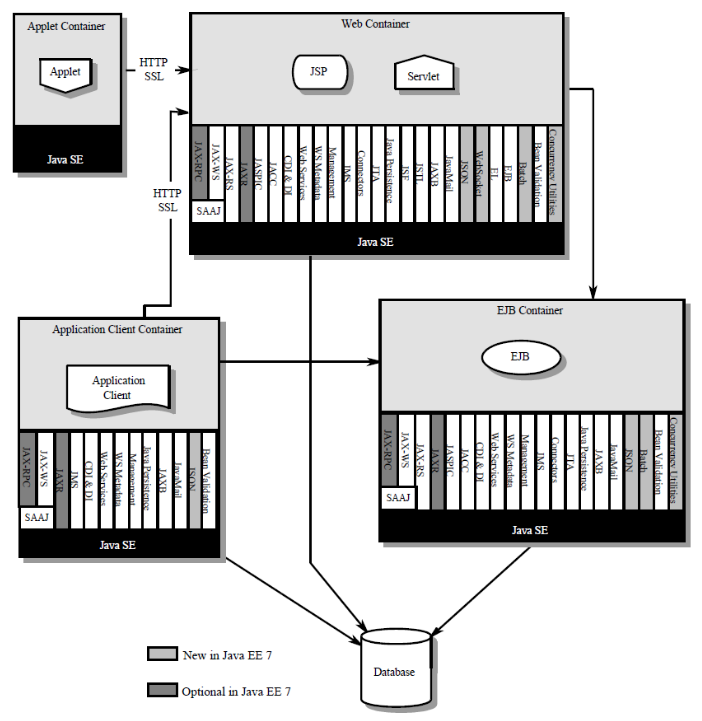
\includegraphics[keepaspectratio=true,height=20\baselineskip]{container_types.png}
    \caption{Verschiedene Container- und Anwendungs-Typen}
    \label{fig:container_types}
\end{figure}

Applikationsserver können entwerder als Full-Profile oder aber als Web-Profile installiert werden. Das Full-Profile enthält alle Container- und Anwendungs-Typen, während das Web-Profil zwar leichter ist, aber auch weniger Funktionen bereitstellt, sondern nur diese, die bei einfacheren Infrastrukturen benötigt werden (so ist z.B. JMS nicht inbegriffen im Web-Profile, da es normalerweise erst bei komplexeren Infrastrukturen benötigt wird)


\section{High Availability (JGroups)}

\section{Web-Tier}

\section{EJB-Tier}

EJB steht für "Enterprise Java Bean". Sie sind serverseitige Komponenten, die die Business-Logik einer Applikation zusammenfassen. Sie  stellen Services wie z.B. Transationen, Logging oder Security zur Verfügung. \\
Grundsätzlich wird zwischen vier Arten von Beans unterschieden:

\subsection{Typen von EJBs}
\begin{description}
    \item[@Stateless: ] Stellen zustandlose Dienste zur Verfügung (Jede Anfrage wird als neue Anfrage behandelt, es wird nichts zwischengespeichert)
    \item[@Stateful: ] Stellen zustandsbehaftete Dienste zur Verfügung (Es werden gewisse Informationen zwischengespeichert, die bei späteren Anfragen wiederverwendet werden können)
    \item[@Singleton: ] Existiert genau einmal in der gesamten Applikation und stellt einen zustandsbehafteten Service zur Verfügung
    \item[@MessageDriven: ] Reagieren auf asynchrone Messages
\end{description}

Diese Beans sind nicht automatisch von überall her sichtbar und können auch nicht von überall her benutzt werden. Es muss eine Sichtbarkeit festgelegt werden:

\begin{description}
    \item[@Local: ] Von allen Komponenten innerhalb derselben JVM sichtbar (Es können mehrere Applikationen auf einem Applikationsserver laufen. Diese können nun alle auf diese Bean zugreifen)
    \item[@Remote: ] Auch für Anwendungen sichtbar, die ausserhalbe der JVM laufen
    \item[@LocalBean: ] Nur innerhalb des EAR-Projekts der Applikation sichtbar, also ausschliesslich innerhalb dieser Applikation
\end{description}
Typen von EJBs


\section{JEE Security}

\section{Messaging Services}

\section{REST}

\section{JNDI \& LDAP}

\section{CDI}

\section{Architektur \& Agiles Vorgehen}

\end{document}
